\chapter{Image reconstruction}
\label{ch:image-reconstruction}

\begingroup
\raggedbottom

\draftnote{\textbf{STATUS (2026-11-25).} Drafted to the supervisor's piecewise-linear account (meeting 2026-11-24): the opening (orientation, view extraction, $K$ vs.\ $N$), \cref{sec:aberrations-as-shifts} P1--P5 with \cref{fig:aberration-segments}, and the bridge into \cref{sec:global-local-alignment}. \textbf{Budget:} about 1.92 pages plus two figures (raised from 1.85 on 2026-11-25 to keep the walk-through of \cref{fig:single-view-alignment}); the aberration section about 316 words (departure table, 2026-11-25). \textbf{Waiting on:} the supervisor's verdict on the section and its figure (next meeting); the view-grid pointer to \cref{sec:app-view-extraction} was added 2026-11-25. (\cref{fig:single-view-alignment} provenance recorded 2026-11-25: acquired 2026-06-16, capture confirmed, \texttt{algo} commit 8cb681b; see \texttt{research-context/result-provenance/fig\_alignment\_evolution.yaml}.)\textbf{History:} \texttt{planning/writing-log.md}, 2026-11-23 to 2026-11-25; the retired Shack--Hartmann text is in \texttt{supporting-material/drafts/ch05-shack-hartmann-legacy-2026-11-24.md}.}

% Opening rewritten 2026-11-25 (author: ease the reader in). View extraction and the K-N note moved to the start of the global-and-local section the same day; the assumptions sentence sits after the two stages.
Chapter~\ref{ch:light-field-microscope} showed that one FLFM capture holds many small images of the scene, one per lenslet, each seen through a different part of the pupil. When the light crosses an aberrating sample, these views no longer line up: the same structure appears at slightly different positions in each. This chapter explains where these displacements come from and how we undo them to recover a single two-dimensional image. In short, we align the views and average them, as in classical light-field rendering \cite{levoyHanrahan1996lightFieldRendering}.

\section{Aberrations as shifts}
\label{sec:aberrations-as-shifts}

% P1 rewritten 2026-11-25 (author: simpler, with a link to P2).
Each view images the scene through one segment of the pupil, like a small-aperture microscope (\cref{fig:flfm-path}). Since fluorescent emitters are incoherent, a view is the sum of the images of the individual emitters \cite{guo2019fourierLightField}. We assume a flat scene, with all emitters within about $\Delta z_{LF}$ of one plane, so that their depth differences shift them between views by less than one resolution element (\cref{sec:factors-of-n}). Without aberration, the views of such a scene differ only by one shift per view. To see how an aberration changes this, we follow the light of one emitter to the lenslets.

% P2-P4 drafted 2026-11-25 in the supervisor's piecewise-linear terms (meeting 2026-11-24); they replace the text moved from Chapter 3. Figure fig:aberration-segments (approved 2026-11-25, departure table) drawn 2026-11-25 in figures/ch04/aberration-segments.tex.
In a uniform medium, an in-focus emitter's light reaches the back pupil as a plane wave, with a linearly varying phase. Refractive-index variations in the sample distort this phase (\cref{fig:aberration-segments}a). Within each view's segment, we approximate the phase by a linear ramp of the same mean slope. This ramp tilts the segment's light and so shifts the whole view \cite{ji2010adaptiveOpticsPupilSegmentation}. The lenslets therefore fit the wavefront piecewise linearly.

Defocus, for example, adds a quadratic phase, whose slope grows linearly with distance from the pupil center. Each view therefore shifts in proportion to its position, the parallax of \cref{sec:factors-of-n}. Since a single depth sets all these shifts, refocusing undoes them \cite{levoy2009recordingControlling4d}. A general aberration also shifts every view, but by amounts no single parameter predicts, so each shift must be measured.

A conventional microscope adds the light of all segments, so these shifted copies blur together. The FLFM records the views apart, so shifting them back before averaging removes the aberration, up to the phase variation within each segment. The price is resolution: each view resolves only $\Delta x_{LF}=N\Delta x_o$, and following the wavefront with more, smaller segments coarsens every view.

The views also reveal aberrations that vary across the field. In a complex, heterogeneous sample, an emitter elsewhere follows a different path and meets a different aberration (\cref{fig:aberration-segments}b), so its views shift differently. Measuring the shifts locally, within bounded search ranges, undoes this variation too.

\begin{figure}[tbp]
    \centering
    \resizebox{\textwidth}{!}{% Aberrations as a piecewise-linear fit of the wavefront (Chapter 4,
% sec:aberrations-as-shifts). After the supervisor's drawing at the
% 2026-11-24 meeting; figure approved 2026-11-25 (departure table).
% Redrawn 2026-11-25 (author): the wavefronts sit on the system diagram;
% polished the same day (larger labels, the fit made to stand out).
% Each panel: an emitter in a heterogeneous sample sends spherical
% wavefronts that are clean near the emitter and distorted after the
% inclusions; behind the objective the wavefront is nominally plane; at the
% lenslets (N = 7 segments) the ideal (dashed), real (thin) and
% piecewise-linear approximated (thick) wavefronts are superimposed. The
% approximation joins the real wavefront at the segment ends, so each
% piece has the segment's mean slope. (a) and (b): two emitters in the same
% sample, with different distortions and fits. Schematic; the distortions
% are made up and enlarged at the lenslets.
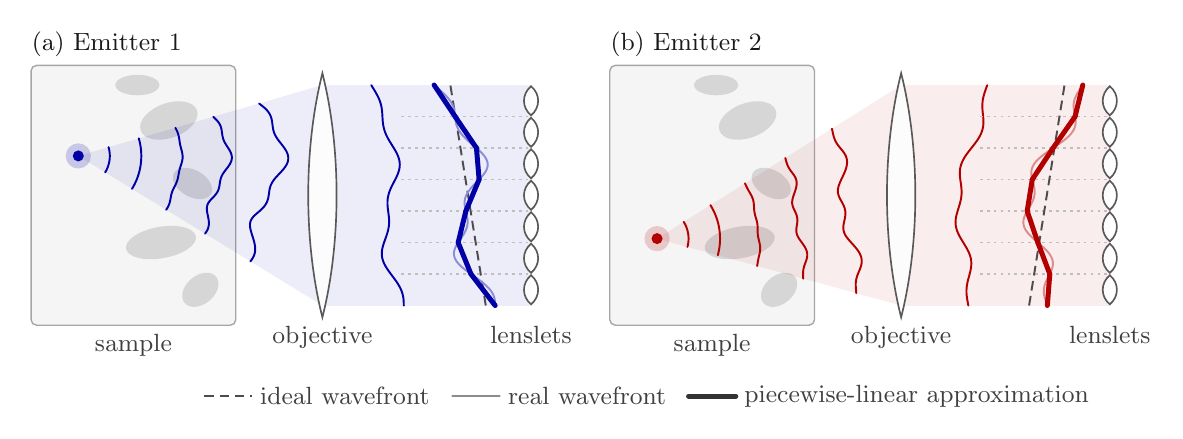
\begin{tikzpicture}[
    x=1cm,y=1cm,
    font=\small,
    lab/.style={font=\small,text=black!75,inner sep=1.5pt,align=center},
    title/.style={font=\small,text=black!90,inner sep=1.5pt},
    ideal/.style={draw=black!70,line width=0.7pt,dash pattern=on 3.5pt off 2pt},
    real/.style={line width=0.7pt,line cap=round,line join=round},
    approx/.style={line width=1.8pt,line cap=round,line join=round},
    lens/.style={draw=black!65,line width=0.6pt,fill=white,fill opacity=0.85}
]
% ---- shared geometry (cm; not to scale) ----
\def\sw{2.6}      % sample width
\def\xe{0.6}      % emitter depth in the sample
\def\xl{3.7}      % objective
\def\hl{1.4}      % half-height of the beam at the objective and the pupil
\def\xm{4.55}     % a wavefront between the objective and the lenslets
\def\xw{5.55}     % the wavefront at the lenslets
\def\xa{6.35}     % lenslet array
\def\s{0.4}       % wavefront displacement per unit of phase
\def\sl{0.75}     % the same at the lenslets, enlarged for visibility
% aberration part of the wavefront, u in [-1,1] across the beam. The last
% term vanishes at the segment ends (u = -1 + 2k/7), so it leaves the fit
% unchanged and bows the real wavefront within each segment.
\def\abA(#1){(0.30*sin(deg(4*(#1)+0.3))+0.12*sin(deg(3.5*pi*((#1)+1))))}
\def\abB(#1){(-0.33*cos(deg(3.5*(#1)))-0.12*sin(deg(3.5*pi*((#1)+1))))}

\foreach \ox/\ye/\tilt/\ab/\c/\title in
    {0/0.5/-0.3/\abA/blue!65!black/{(a) Emitter 1},
     7.35/-0.55/0.3/\abB/red!70!black/{(b) Emitter 2}} {
\begin{scope}[shift={(\ox,0)}]
    % ---- sample and its refractive-index variations ----
    \fill[black!4,rounded corners=2pt] (0,-1.65) rectangle (\sw,1.65);
    \foreach \cx/\cy/\rx/\ry/\ang in {1.75/0.95/0.38/0.22/20, 2.05/0.15/0.27/0.17/-30,
            1.65/-0.6/0.45/0.2/10, 2.15/-1.2/0.26/0.18/40, 1.35/1.4/0.28/0.13/0}
        \fill[black!16,rotate around={\ang:(\cx,\cy)}] (\cx,\cy) ellipse ({\rx} and {\ry});
    \draw[black!35,line width=0.5pt,rounded corners=2pt] (0,-1.65) rectangle (\sw,1.65);
    \node[title,anchor=south west] at (-0.05,1.7) {\title};

    % ---- light: cone to the objective, collimated beam to the lenslets ----
    \fill[\c,opacity=0.07] (\xe,\ye) -- (\xl,\hl) -- (\xl,-\hl) -- cycle;
    \fill[\c,opacity=0.07] (\xl,-\hl) rectangle (\xa,\hl);
    \pgfmathsetmacro{\aT}{atan2(\hl-\ye,\xl-\xe)}
    \pgfmathsetmacro{\aB}{atan2(-\hl-\ye,\xl-\xe)}

    % ---- spherical wavefronts: clean near the emitter, distorted after
    % the inclusions (the distortion grows with the path through them) ----
    \foreach \r/\amp in {0.4/0, 0.8/0, 1.3/0.15, 1.85/0.6, 2.5/1} {
        \draw[\c,real,samples=90,domain=0:1]
            plot ({\xe+(\r+\amp*\s*\ab(2*\x-1))*cos(\aB+\x*(\aT-\aB))},
                  {\ye+(\r+\amp*\s*\ab(2*\x-1))*sin(\aB+\x*(\aT-\aB))});
    }
    \fill[\c,opacity=0.18] (\xe,\ye) circle (0.16);
    \fill[\c] (\xe,\ye) circle (0.07);

    % ---- objective (biconvex) ----
    \draw[lens] (\xl,-1.55) .. controls (\xl+0.24,-0.6) and (\xl+0.24,0.6) .. (\xl,1.55)
                           .. controls (\xl-0.24,0.6) and (\xl-0.24,-0.6) .. cycle;

    % ---- behind the objective: nominally plane, but distorted ----
    \draw[\c,real,samples=90,domain=-1:1]
        plot ({\xm+\s*(\tilt*\x+\ab(\x))},{\hl*\x});

    % ---- at the lenslets: segments, ideal, real, approximation ----
    \foreach \k in {1,...,6}
        \draw[black!25,line width=0.4pt,dash pattern=on 1pt off 1.5pt]
            (\xw-0.85,{-\hl+2*\hl*\k/7}) -- (\xa,{-\hl+2*\hl*\k/7});
    \draw[ideal] ({\xw-\sl*\tilt},-\hl) -- ({\xw+\sl*\tilt},\hl);
    \draw[\c!45,real,samples=140,domain=-1:1]
        plot ({\xw+\sl*(\tilt*\x+\ab(\x))},{\hl*\x});
    \foreach \k in {0,...,6} {
        \pgfmathsetmacro{\ua}{-1+2*\k/7}
        \pgfmathsetmacro{\ub}{-1+2*(\k+1)/7}
        \pgfmathsetmacro{\pa}{\tilt*\ua+\ab(\ua)}
        \pgfmathsetmacro{\pb}{\tilt*\ub+\ab(\ub)}
        \draw[\c,approx] ({\xw+\sl*\pa},{\hl*\ua}) -- ({\xw+\sl*\pb},{\hl*\ub});
    }

    % ---- lenslet array in the back pupil: N = 7 segments ----
    \pgfmathsetmacro{\pw}{2*\hl/7}
    \foreach \k in {0,...,6} {
        \pgfmathsetmacro{\ya}{-\hl+\pw*\k+0.015}
        \pgfmathsetmacro{\yb}{-\hl+\pw*(\k+1)-0.015}
        \draw[lens] (\xa,\ya) .. controls (\xa+0.12,\ya+0.25*\pw) and (\xa+0.12,\yb-0.25*\pw) .. (\xa,\yb)
                             .. controls (\xa-0.12,\yb-0.25*\pw) and (\xa-0.12,\ya+0.25*\pw) .. cycle;
    }

    % ---- labels ----
    \node[lab,anchor=north] at (\sw/2,-1.7) {sample};
    \node[lab,anchor=north] at (\xl,-1.6) {objective};
    \node[lab,anchor=north] at (\xa,-1.6) {lenslets};
\end{scope}
}
% ---- legend ----
\begin{scope}[shift={(2.2,-2.55)}]
    \draw[ideal] (0,0) -- (0.6,0);
    \node[lab,anchor=west] at (0.65,0) {ideal wavefront};
    \draw[black!45,real] (3.15,0) -- (3.75,0);
    \node[lab,anchor=west] at (3.8,0) {real wavefront};
    \draw[black!80,approx] (6.15,0) -- (6.75,0);
    \node[lab,anchor=west] at (6.8,0) {piecewise-linear approximation};
\end{scope}
\end{tikzpicture}
}
    \caption[Aberrations as a piecewise-linear fit of the wavefront.]{Aberrations as a piecewise-linear fit of the wavefront. An emitter in a heterogeneous sample sends out spherical wavefronts, which are distorted as they cross refractive-index variations (gray). Behind the objective the wavefront would be plane; instead it reaches the lenslets in the back pupil, one segment per view ($N=7$, gray lines), still distorted. There, the ideal (dashed), real (thin) and approximated (thick) wavefronts are superimposed: within each segment, the approximation is a tilted plane with the segment's mean slope, which shifts that view. (a)~Emitter~1. (b)~Emitter~2, elsewhere in the same sample, meets a different aberration and gets a different fit, so the shifts vary across the field. Schematic, not to scale; the distortions are illustrative and enlarged at the lenslets.}
    \label{fig:aberration-segments}
\end{figure}

\section{Global and local alignment}
\label{sec:global-local-alignment}

Correction therefore takes two steps: one shift per view, then a shift per pixel. These are the global and local stages of the reconstruction.

% View extraction moved here 2026-11-25 (author): the notation is first used by the two stages.
Both stages work on the views as separate images, so we first cut the sensor frame into a $K\times K$ grid of views, one per lenslet. Note that $K$ counts the views we extract along each side, while $N$ (\cref{sec:flfm-principle}) counts the whole views across the pupil in the optical design; in our acquisitions $K=N=7$ (\cref{sec:app-view-extraction}). We denote by $V_{ij}(y,x)$ view $(i,j)$, with $i,j\in\{1,\ldots,K\}$, at pixel row $y$ and column $x$ of the $H\times W$ grid $\Omega$ shared by all views. We use the FLFM notation of Guo et al.~\cite{guo2019fourierLightField}.

In the global stage, the central view $V_{cc}$ is the reference. Cross-correlation over a bounded range of integer shifts $s$ gives one translation for each entire view,

\begin{equation}
    d^g_{ij}=\operatorname*{arg\,max}_{s}\sum_{(y,x)\in\Omega}V_{cc}(y,x)\,V_{ij}(y-s_y,x-s_x).
\end{equation}

Translating each view by $d^g_{ij}$ gives the aligned views $V^g_{ij}$. Their pixelwise mean over all $K^2$ views is the intermediate global-stage average $G$.

A single translation cannot follow displacements that vary across a view, so the local stage uses $G$ as the reference for every aligned view. At each pixel, a bounded search, possibly in steps finer than one pixel, selects the displacement $d^\ell_{ij}(y,x)$ with the highest match score between $G$ and $V^g_{ij}$, whose intensities may first be raised to a power. The score is the Gaussian-weighted product of the two images around the pixel, divided by a Gaussian-weighted local intensity normalization, and each pixel's displacement is selected independently. Each aligned view is then warped by its displacement field, and the mean over all warped views is the final rectified image,

\begin{equation}
    V^\ell_{ij}(y,x)=\operatorname{Interp}\!\left(V^g_{ij},(y,x)-d^\ell_{ij}(y,x)\right),
    \qquad I_{\mathrm{rect}}(y,x)=\frac{1}{K^2}\sum_{i=1}^{K}\sum_{j=1}^{K}V^\ell_{ij}(y,x).
\end{equation}

Besides a flat scene (\cref{sec:aberrations-as-shifts}), both stages assume that corresponding structure is visible in enough views, that the shifts fall within the search bounds, and that the central view is a suitable reference.

% Walk-through rewritten 2026-11-25 (author: use the figure, do not repeat its caption; lead with the point, not the numbers, which stay in the caption).
Figure~\ref{fig:single-view-alignment} shows why one shift per view is not enough. Global alignment moves both regions of a view by the same shift (B), yet what remains of their displacement points in opposite directions (E). No single translation can correct both, but local refinement brings each region into register with $G$ (F). Comparing $G$ with $I_{\mathrm{rect}}$ from the same run therefore isolates what local refinement adds. Appendix~\ref{app:reconstruction-method} gives the complete method and the exact local score.

\begin{figure}[p]
    \centering
    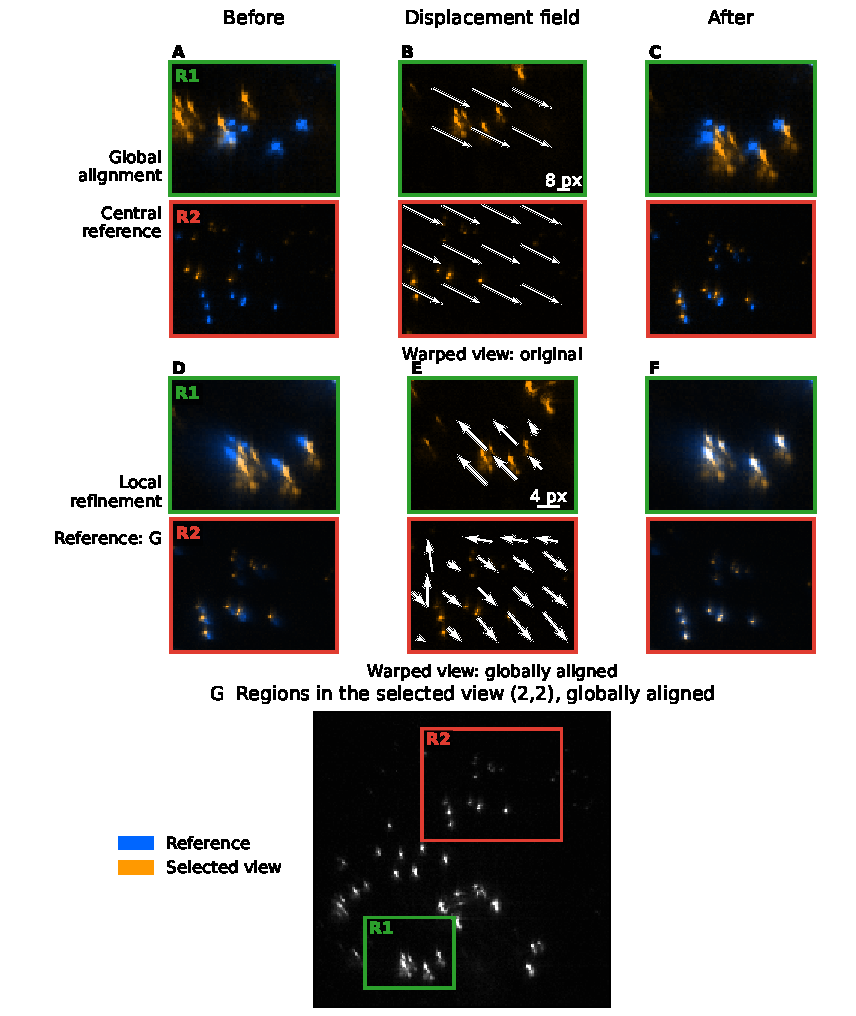
\includegraphics[width=0.9\linewidth]{figures/ch04/alignment-evolution.pdf}
    \caption[Image evolution and warping through both alignment stages.]{Image evolution and warping for view $(2,2)$ in a $7\times7$ FLFM acquisition of fluorescent beads under gel eyedrops (dense10 run; one-based view indices). Each panel in (A--F) shows two regions of the same view, R1 (84$\times$67 px) above R2 (132$\times$106 px, shown at lower magnification). (A--C) Global alignment uses the original central reference. (D--F) Local refinement uses the global-stage average $G$, including the selected view. The left and right columns overlay the reference (blue) and selected view (orange) before and after correction; C and D contain the same aligned view with different references. Middle panels show the displacement fields as arrows over the view being warped (original in B, globally aligned in E), from $p-m\,d(p)$ to the output position $p$, so each arrow points in the direction the content moves ($m=1$ in B, $m=4$ in E; the bars show 8 px in B and 4 px in E at that scale). Global alignment applies the same shift, $(16,32)$ px (row, column), in both regions; the mean local displacement is $(-4.6,-4.5)$ px in R1 and $(1.6,2.7)$ px in R2. (G) Both regions in the globally aligned view, cropped to the area around them. Linear display limits are shared, except that the reference $G$ in (D--F) uses an upper limit $0.55$ times as high to offset the dimming from averaging; all images use nearest-neighbor display; reconstruction uses linear interpolation. The regions are illustrative.}
    \label{fig:single-view-alignment}
\end{figure}

\clearpage
\endgroup
